\chapter{Whirl current}
%

% - Purpose & Problem description:
%     These first two parts give reader short details about the test case,
%     the physical phenomena involved and specify how the numerical solution will be validated
%
\section{Purpose}
%
This test case should make it possible to check that the effects of refraction
by the current are properly taken into account by Tomawac 7.0. The distorsion
of a wave spectrum as it reaches a whirl current zone like those observed along
the Norwegian coasts \cite{Mathiesen1987}
%
\section{Description of the problem}
%
This test case is derived from the Mathiesen's results \cite{Mathiesen1987}.
Equivalent results can be found in \cite{Tolman1991} and \cite{Hubbert1991}. The
spatial domain is a 80 km-sided square (see Figure \ref{current}). A circular,
origin-centered whirl current is considered ; it is modelled as follows. Is
tangential velocity is zero at the origin and linearly increases up to $r=r_1$
as per :
$$
u(r) = u_l\frac{r}{r_l} \mbox{ for } r\le r_l\le r_0
$$
Then, that velocity follows a Gaussian profile:
$$
u(r)=u_{max} \exp \left( -\left(\frac{r-r_0}{br_0}\right)^2 \right) \mbox{ for } r > r_l
$$
Both continuity and derivability for u lead to:
$$
%\left.
%\begin{array}{ll}
\frac{r_l}{r_0}=\frac{1+ \sqrt{1-2b^2}}{2} %\\[6pt]
%\frac{u_l}{u_{max}}= \exp \[ -\left( \frac{r_l-r_0}{br_0} \right)^2 \]
%\end{array}
%\right.
$$
$$
\frac{u_l}{u_{max}}= \exp \left( -\left(\frac{r_l-r_0}{br_0}\right)^2 \right)
$$
The following values were adopted in the computations: $u_{max}=1m/s$,
$r_0=10km$ and $b=0.3$.
% - Reference:
%     This part gives the reference solution we are comparing to and
%     explicits the analytical solution when available;
%
%
\begin{figure} [H]
\centering
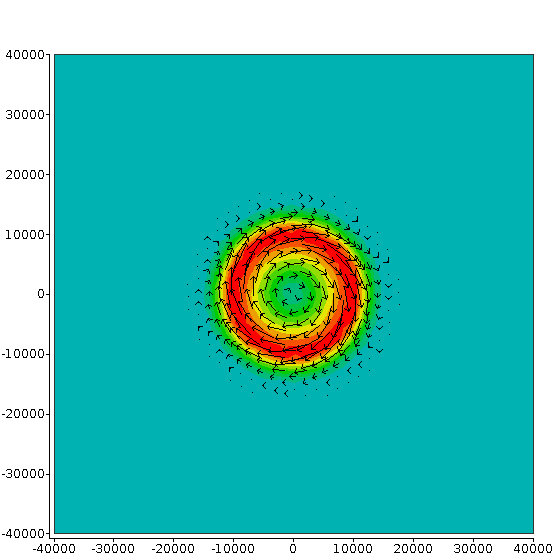
\includegraphics[width=0.85\textwidth]{current.png}
 \caption{whirl current}
\label{current}
\end{figure}
The model as developped by Mathiesen is a refraction model that computes the
orthogonal waves through a conventional ray method. The results it provides for
the 0.1\ Hz frequency are displayed on Figure \ref{ray}. Many orthogonal
crossings can be observed.
\begin{figure} [!h]
\centering
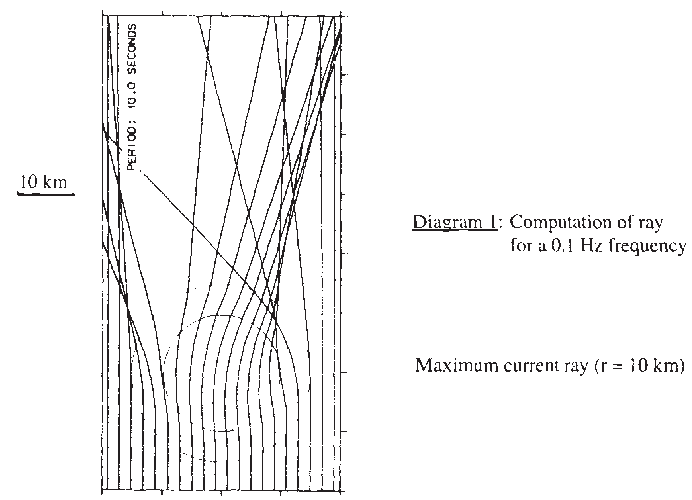
\includegraphics[width=0.85\textwidth]{diagram.png}
 \caption{Computation of rays}
\label{ray}
\end{figure}

\section{Initial and Boundary Conditions}

That method of rays can be implemented  either forwards (as on Figure
\ref{ray}), or backwards, then knowing the arrival point of an orthogonal, it
provides the starting point. A whole wave spectrum can be reconstructed by
multiplying the computations of this kind. The incident spectrum as prescribed
by \cite{Mathiesen1987} is as follows :
$$
S(f,\theta)=S(f)D(f,\theta)
$$
In that expression $S(f)$ is a frequency spectrum of the classical Jonswap type, where the peak frequency $f_p$ is set to 0.1 Hz.
$D(f,\theta)$ is a Gaussian distribution:
$$
D(f,\theta)=\frac{\exp\left(-\frac{(\theta-\theta_m)^2}{2\sigma_0^2} \right)}{\sqrt{2\pi}\sigma_0}
$$
$\theta_m$ is the mean direction of the incident waves (here $\theta_m=0$) and
$\sigma_0$ is given by the following relationship.
$$
\left.
\begin{array}{ll}
\sigma_0= \sigma_{0p}\left(\frac{f}{f_p}\right)^{-2.03}\mbox{ if }f<f_p \\[6pt]
\sigma_0= \sigma_{0p}\left(\frac{f}{f_p}\right)^{1.04}\mbox{ if } f \ge f_p
\end{array}
\right.
$$
where $\sigma_{0p}$, the directional spread at the peak, is 25 in our case.
This spectrum is imposed on the East South and West boundaries while the North boundary is free.

The initial spectrum is null.
%\subsection{Reference}
%

% - Physical parameters:
%     This part specifies the geometry, details all the physical parameters
%     used to describe both porous media (soil model in particularly) and
%     solute characteristics (dispersion/diffusion coefficients, soil <=> pollutant interactions...)
%
%
% - Geometry and Mesh:
%     This part describes the mesh used in the computation
%
%
\section{Geometry and Mesh}
%
The mesh is made of 1876 nodes and 3590 triangles and is shown Figure \ref{mail}
\begin{figure} [H]
\centering
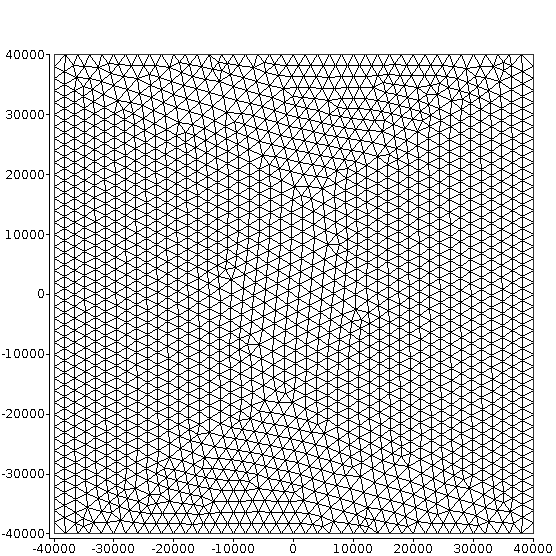
\includegraphics[width=0.85\textwidth]{maill.png}
 \caption{Mesh of the domain}
\label{mail}
\end{figure}

% - Initial and boundary conditions:
%     This part details both initial and boundary conditions used to simulate the case
%
%

\section{Numerical parameters}
%
Time duration is 60000\ s, time step is equal to 1200\ s, the spectro-angular mesh
has 48 angles and 25 frequences spread on a geometric progression common ratio
1.1 with a minimum of  0.04177248.
% - Results:
%     We comment in this part the numerical results against the reference ones,
%     giving understanding keys and making assumptions when necessary.
%
%
\section{Results}
%
On figure \ref{measurepts}, we present the amplification factor of the heigth
due to the current. We can notice two different zones at the center of the
domain where there is a strong modification of the heigth. One zone where the
heigth is raising (till 35\%) when the swell is opposed to the current, and one
zone where the heigth is decreasing (till 20\%) where swell and current are in
the same direction. On the other parts of the domain, modifications are less than
5\%. Those results are coherent with the ray calculus presented on Figure
\ref{ray} since on the two zones we denote orthogonal crossing.

In his paper, Mathiesen \cite{Mathiesen1987} defines 8 points shown on
Figure \ref{measurepts}. On these points he gives the energy angular spread at
0.1 Hz (frequency peak of the incident spectrum). We compare this spread to the
one obtained by Tomawac on Figure \ref{repartang}. We can denote that the
results are very closed to Mathiesen results especially on points 4 and 7.
Notice that Mathiesen took an angular discretisation of 2.5 when our is of 7.5.

\begin{figure} [H]
\centering
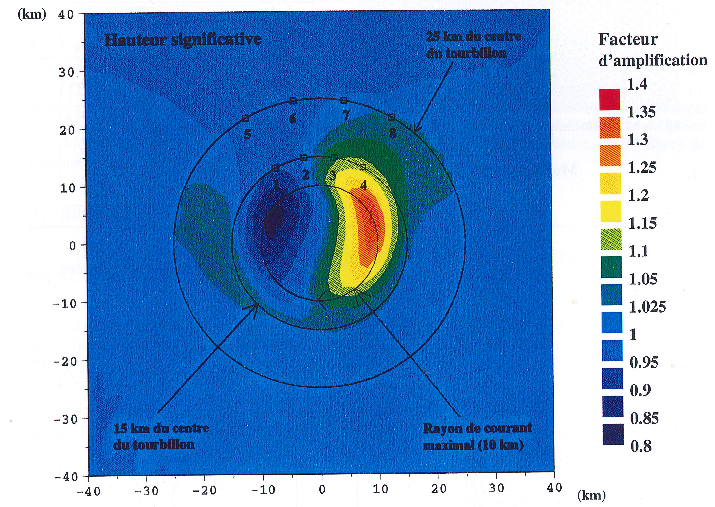
\includegraphics[width=0.85\textwidth]{whirlcurrentpoints.png}
 \caption{significative heigth and positions of the measurement points}
\label{measurepts}
\end{figure}


\begin{figure} [H]
\centering
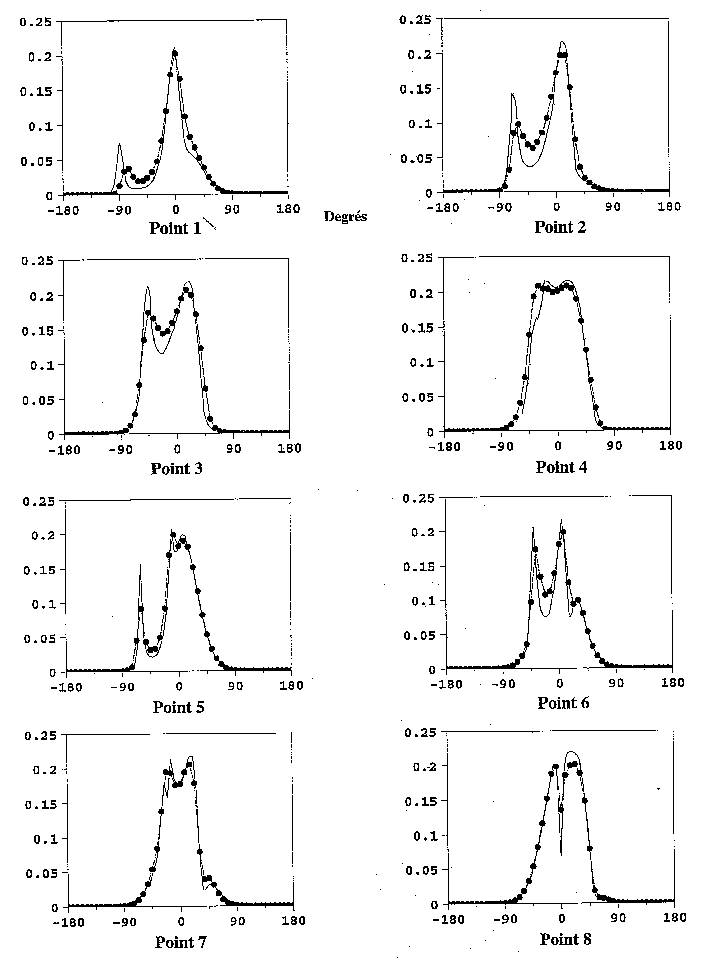
\includegraphics[width=0.85\textwidth]{repartangulaire.png}
 \caption{Comparison of the angular spread at 0.1 Hz between Tomawac and Mathiesen}
\label{repartang}
\end{figure}

\begin{figure} [H]
\centering
\includegraphicsmaybe{[width=0.85\textwidth]}{../img/results.png}
 \caption{significative heigth of the last calculation}
\label{resultswhirl}
\end{figure}

\section{Conclusion}
This test case showed on a realistic case of refraction of current that Tomawac
gives suitable results compared to fine results.
